\documentclass[10pt]{article}
\usepackage{graphicx}
\usepackage{subcaption}
\usepackage[T1]{fontenc}
\usepackage{amsmath}
\usepackage{lipsum}
\usepackage{amsfonts}
\usepackage{hyperref}
\usepackage{mathtools}
\providecommand\given{}
\usepackage[utf8]{inputenc}
\usepackage[letterpaper,margin=1in]{geometry}
\usepackage[parfill]{parskip}

\def\therefore{\boldsymbol{\text{ }
\leavevmode
\lower0.4ex\hbox{$\cdot$}
\kern-.5em\raise0.7ex\hbox{$\cdot$}
\kern-0.55em\lower0.4ex\hbox{$\cdot$}
\thinspace\text{ }}}

\vspace{-8ex}
\date{}

\graphicspath{ {./figs/} }

\begin{document}

\title{\textbf{\Large{\textsc{ECE410:} Linear Control Systems}} \\ \Large{Lab 1 Report: NL Sims?} \\ \textbf{\small{PRA101}}\vspace{-0.3cm}}
\author{Pranshu Malik, Varun Sampat \\ \footnotesize{1004138916}, \footnotesize{1003859602}\vspace{-3cm}}

\maketitle

\section{Introduction}
We have a system $G(s)$ that is very nice.


\subsection{Numerical integration Graphs and Evaluation}
This section models the system using the differential equations provided in the lab handout, and solves the DE by numerical integration. 

Recall, the given non-linear function was:
\begin{center}
   \begin{math}
    \dot{x} = f(x, t) = 
        \begin{bmatrix}
        x_2\\
        -\frac{g sin(x_1)}{l} - \frac{cos(x_1) u(t)}{ml}
        \end{bmatrix}
    \end{math} 
\end{center}

There were two initial conditions of interest:
\begin{center}
    1.
    \begin{math}
     x^0_1 = 
     \begin{bmatrix}
     0\\ \sqrt{g/l}
     \end{bmatrix}
    %  ;
    %  u^0_1 = 0
    \end{math}
\end{center}

\begin{center}
    2. 
    \begin{math}
     x^0_2 = 
     \begin{bmatrix}
     0\\1.99 \sqrt{g/l}
     \end{bmatrix}
    %  ;
    %  u^0_2 = 0
    \end{math}
\end{center}

Note, $x_1 = \theta$, and $x_2 = \dot{\theta}$. 
$\theta = 0$, but $\dot{\theta}$ is a non-zero value. This is similar to providing the pendulum with an initial velocity from its rest position (equilibrium at $\theta = 0$) at time $t = 0$.

$u(t) = 0$ for this section, implying the system behaves naturally; there is no forced response.

\subsubsection{Graphs for initial condition 1}
Here are the figures for the initial condition 1:
    
    \begin{figure}[ht]
     \centering
     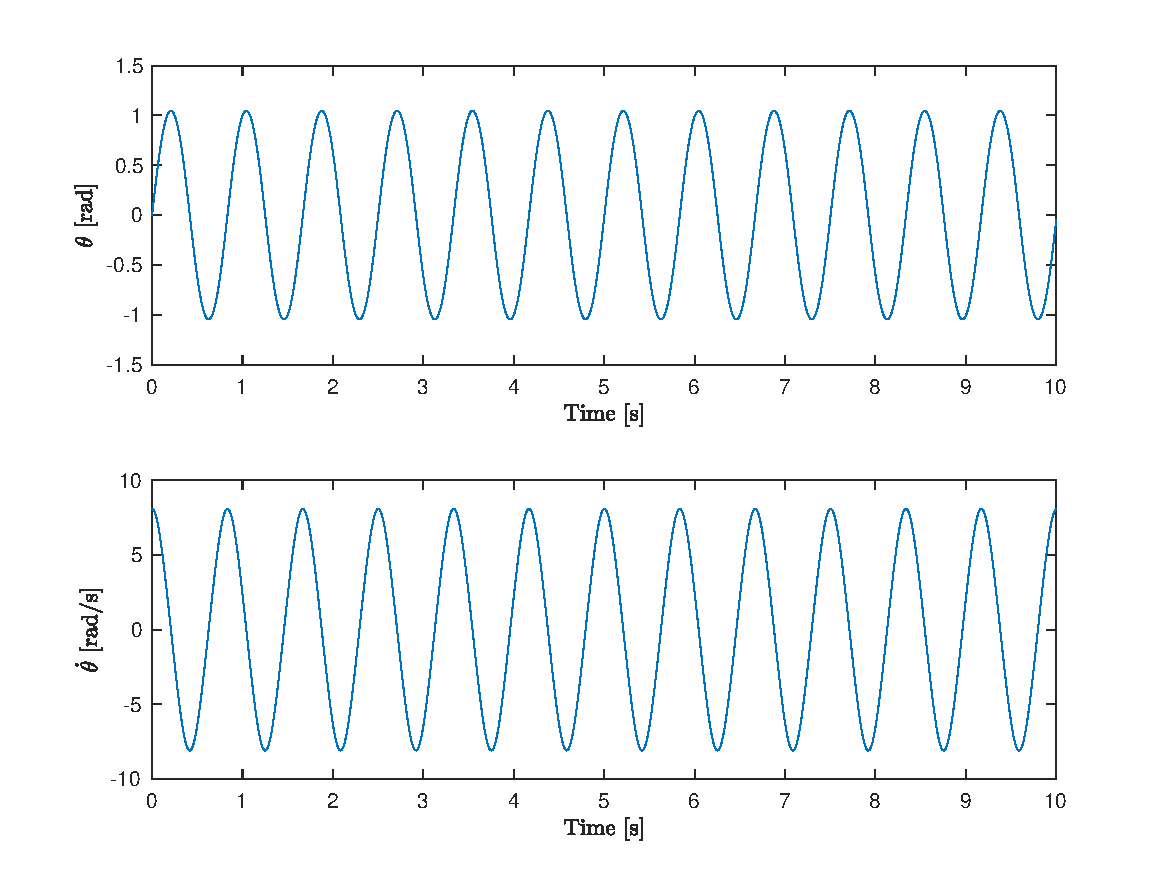
\includegraphics[scale=0.7]{lab1/figs/section3_x0_1_state_evolution.pdf}
     \caption{State Evolution to initial condition 1}
     \label{figure:x_0_1_state_evolution}
    \end{figure}

\end{document}
